%==============================================================================
% Chapitre 62 - Les balles pour fusils lisses
%==============================================================================

\section{Introduction}

Les fusils à canon lisse sont principalement associés aux cartouches à
grenaille.

Ils peuvent toutefois également tirer des projectiles uniques appelés
couramment balles.

Ces munitions permettent d'atteindre des cibles plus importantes tout en
conservant les caractéristiques générales du fusil de chasse.

\begin{aretenir}

Une balle pour fusil lisse est un projectile unique conçu pour être utilisé
dans un canon ne comportant généralement pas de rayures.

\end{aretenir}

\section{Principe général}

Contrairement aux cartouches à grenaille ou à chevrotines, la totalité de la
charge propulsée est constituée d'un seul projectile.

Toute l'énergie est donc concentrée dans une seule masse.

\begin{figure}[htbp]
\centering

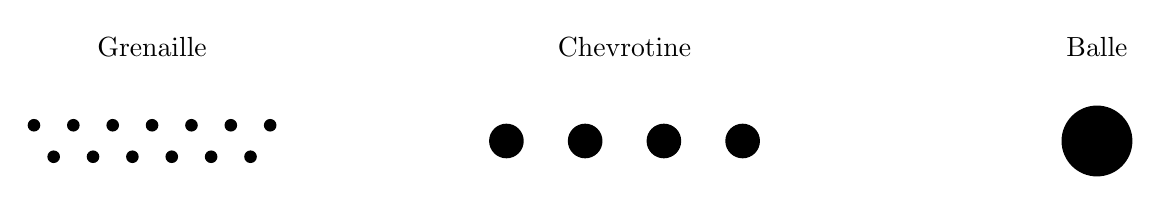
\begin{tikzpicture}

% Grenaille
\node at (0,3) {Grenaille};

\foreach \x in {-1.5,-1,-0.5,0,0.5,1,1.5}
{
    \fill (\x,2) circle (0.08);
}

\foreach \x in {-1.25,-0.75,-0.25,0.25,0.75,1.25}
{
    \fill (\x,1.6) circle (0.08);
}

% Chevrotine
\node at (6,3) {Chevrotine};

\foreach \x in {4.5,5.5,6.5,7.5}
{
    \fill (\x,1.8) circle (0.22);
}

% Balle
\node at (12,3) {Balle};

\fill (12,1.8) circle (0.45);

\end{tikzpicture}

\caption{Comparaison simplifiée entre grenaille, chevrotine et balle unique.}
\label{fig:comparaison_projectiles_chasse}

\end{figure}

\section{Origine historique}

Les premières armes à feu utilisaient principalement des projectiles sphériques tirés dans des canons lisses.

Elles permettaient déjà d'utiliser une même arme pour des usages variés.

\section{Les contraintes du canon lisse}

L'absence de rayures modifie profondément le comportement du projectile.

Les solutions retenues doivent assurer une stabilité suffisante sans recourir
au mécanisme classique de stabilisation gyroscopique.

\section{La balle ronde}

La balle sphérique constitue la forme la plus simple.

Elle fut longtemps utilisée dans les armes anciennes.

\begin{figure}[htbp]
\centering

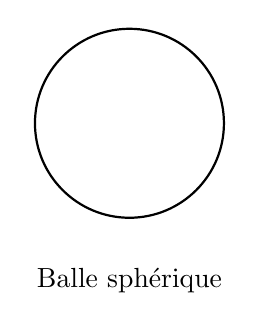
\begin{tikzpicture}

\draw[thick] (0,0) circle (1.2);

\node at (0,-2)
{Balle sphérique};

\end{tikzpicture}

\caption{La balle ronde constitue la forme la plus simple de projectile unique.}
\label{fig:balle_ronde}

\end{figure}

\section{Limites de la balle ronde}

La balle sphérique présente plusieurs inconvénients :

\begin{itemize}
    \item coefficient balistique limité ;
    \item sensibilité aux perturbations ;
    \item portée pratique réduite.
\end{itemize}

\section{La balle Foster}

La balle Foster est l'une des conceptions les plus connues.

Elle possède une cavité arrière importante et des nervures externes
caractéristiques.

\section{Principe de la balle Foster}

La répartition de masse vers l'avant contribue à la stabilité du projectile.

Le comportement peut être comparé à celui d'un volant de badminton.

\begin{figure}[htbp]
\centering

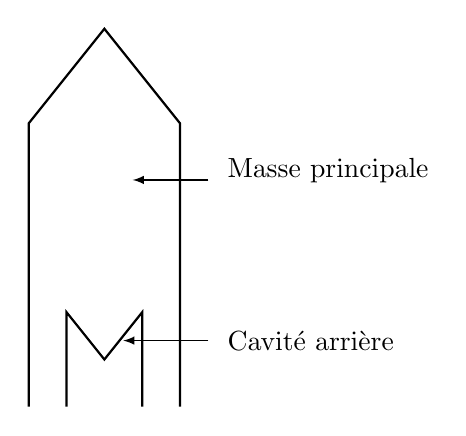
\begin{tikzpicture}[scale=1.2]

\draw[thick]
(0,0)
--
(0,3)
--
(0.8,4)
--
(1.6,3)
--
(1.6,0);

% Cavité
\draw[thick]
(0.4,0)
--
(0.4,1.0)
--
(0.8,0.5)
--
(1.2,1.0)
--
(1.2,0);

\node[right]
at (2,2.5)
{Masse principale};

\draw[-latex]
(1.9,2.4)
--
(1.1,2.4);

\node[right]
at (2,0.7)
{Cavité arrière};

\draw[-latex]
(1.9,0.7)
--
(1.0,0.7);

\end{tikzpicture}

\caption{Principe simplifié d'une balle Foster.}
\label{fig:balle_foster}

\end{figure}

\section{La balle Brenneke}

La balle Brenneke constitue une autre conception largement répandue.

Elle utilise un système différent de stabilisation.

\section{Caractéristiques de la balle Brenneke}

Cette conception comporte généralement :

\begin{itemize}
    \item un projectile massif ;
    \item des nervures extérieures ;
    \item un élément fixé à l'arrière.
\end{itemize}

\begin{figure}[htbp]
\centering

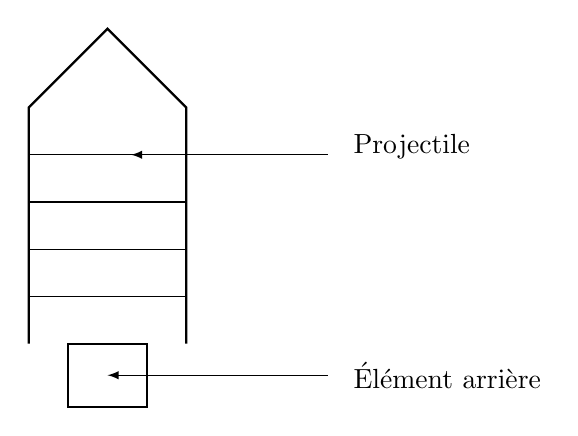
\begin{tikzpicture}

% Corps
\draw[thick]
(0,0)
--
(0,3)
--
(1,4)
--
(2,3)
--
(2,0);

% Nervures
\foreach \y in {0.6,1.2,1.8,2.4}
{
    \draw (0,\y) -- (2,\y);
}

% Élément arrière
\draw[thick]
(0.5,-0.8)
rectangle
(1.5,0);

\node[right]
at (4,2.5)
{Projectile};

\draw[-latex]
(3.8,2.4)
--
(1.3,2.4);

\node[right]
at (4,-0.4)
{Élément arrière};

\draw[-latex]
(3.8,-0.4)
--
(1.0,-0.4);

\end{tikzpicture}

\caption{Principe simplifié d'une balle Brenneke.}
\label{fig:balle_brenneke}

\end{figure}

\section{Les balles sabot}

Certaines munitions utilisent un projectile de diamètre inférieur contenu dans
un sabot.

Le sabot se sépare après la sortie du canon.

\section{Principe du sabot}

Le sabot permet d'adapter le projectile au diamètre du canon pendant la phase
de propulsion.

\begin{figure}[htbp]
\centering

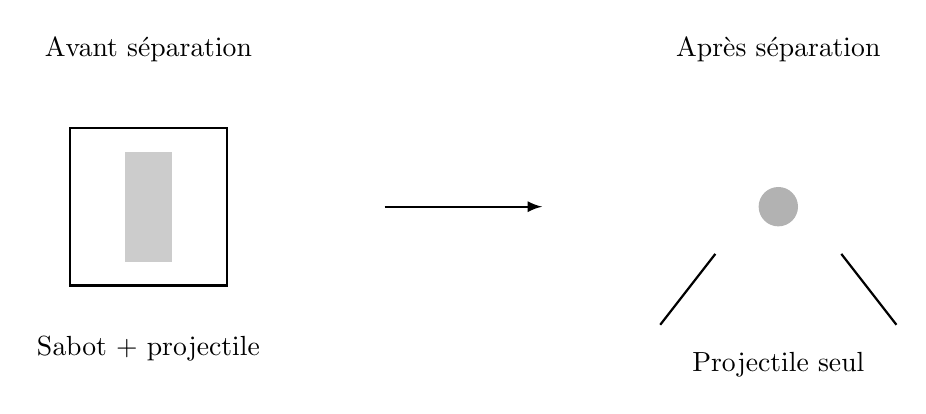
\begin{tikzpicture}

% Avant
\node at (0,3) {Avant séparation};

\draw[thick]
(-1,0)
rectangle
(1,2);

\fill[gray!40]
(-0.3,0.3)
rectangle
(0.3,1.7);

\node at (0,-0.8)
{Sabot + projectile};

% Flèche
\draw[-latex,thick]
(3,1)
--
(5,1);

% Après
\node at (8,3) {Après séparation};

\fill[gray!60]
(8,1)
circle (0.25);

\draw[thick]
(7.2,0.4)
--
(6.5,-0.5);

\draw[thick]
(8.8,0.4)
--
(9.5,-0.5);

\node at (8,-1.0)
{Projectile seul};

\end{tikzpicture}

\caption{Principe simplifié d'une balle sabot.}
\label{fig:balle_sabot}

\end{figure}

\section{Précision}

Les performances en précision dépendent :

\begin{itemize}
    \item du projectile ;
    \item du canon ;
    \item des conditions de tir ;
    \item de la distance.
\end{itemize}

\section{Portée pratique}

Les balles offrent généralement une portée pratique supérieure à celle des
cartouches à grenaille.

\section{Influence du choke}

Selon la conception de la balle, certains chokes peuvent être plus ou moins
adaptés.

Les recommandations du fabricant doivent toujours être respectées.

\section{Applications}

Les balles pour fusils lisses sont utilisées dans différents contextes :

\begin{itemize}
    \item chasse ;
    \item tir sportif ;
    \item usages professionnels spécifiques.
\end{itemize}

\section{Évolution des conceptions}

Les progrès des matériaux et des procédés de fabrication ont permis
l'apparition de projectiles de plus en plus performants.

\section{Vers les matériaux des projectiles}

Les performances d'une balle ne dépendent pas uniquement de sa géométrie.

Le matériau utilisé joue également un rôle important.

Le chapitre suivant examinera les principaux matériaux employés dans les
munitions de chasse.

\section{À retenir}

\begin{aretenir}

\begin{itemize}
    \item Une balle pour fusil lisse est un projectile unique.
    \item Les balles Foster et Brenneke sont parmi les conceptions les plus
          connues.
    \item Les balles sabot utilisent un projectile contenu dans un support
          séparatif.
    \item Les performances dépendent de nombreux paramètres.
    \item Le choix du projectile dépend de l'application recherchée.
\end{itemize}

\end{aretenir}

\begin{figure}[htbp]
\centering

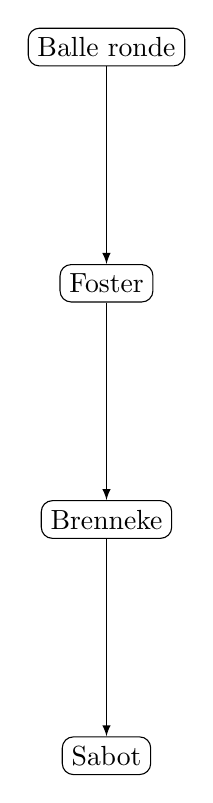
\begin{tikzpicture}

\node[draw,rounded corners]
(R)
at (0,0)
{Balle ronde};

\node[draw,rounded corners]
(F)
at (0,-3)
{Foster};

\node[draw,rounded corners]
(B)
at (0,-6)
{Brenneke};

\node[draw,rounded corners]
(S)
at (0,-9)
{Sabot};

\draw[-latex] (R) -- (F);
\draw[-latex] (F) -- (B);
\draw[-latex] (B) -- (S);

\end{tikzpicture}

\caption{Évolution simplifiée des principales conceptions de balles pour fusils lisses.}
\label{fig:evolution_balles_lisses}

\end{figure}
